\section{Experimental methods}

\paragraph{Measuring converging lenses}
\subparagraph{Lens equation}
\label{chap::lens}

To calculate the focal length $f$ using the lens equation, we need to place an object, in our case a wired net, in front of a monochromatic LED light. 

\begin{figure}[ht]
	\centering
	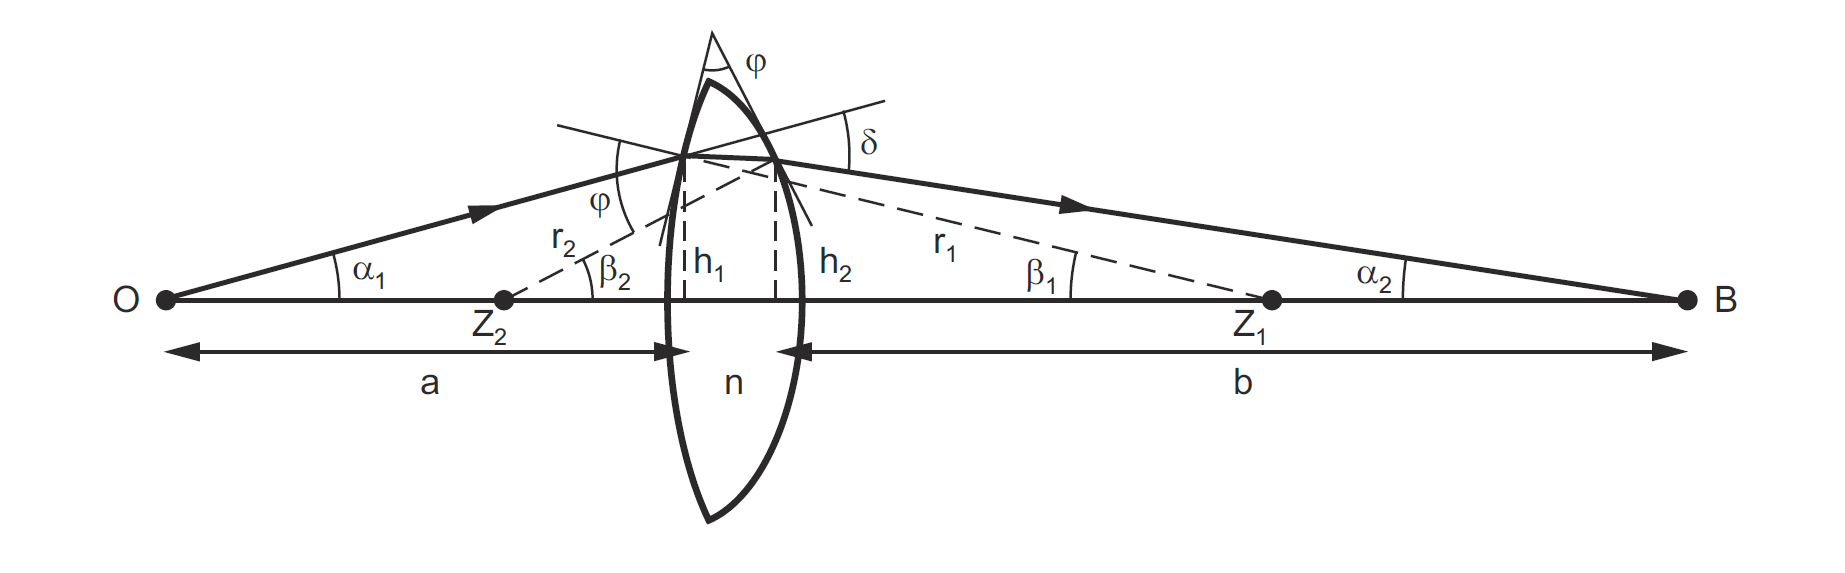
\includegraphics[width=\textwidth]{img/lenseq.PNG}
	\caption{Descriptive image\cite{manual} of the setup to measure the lens with the lens equation.}
	\label{fig::lens}
\end{figure}
The light then passes through the lens we want to measure and the image is projected on to a white screen, as seen in Figure \ref{fig::lens}.
Now the goal is to adjust the position of the lens, so that the image is as sharp as possible.
That gives us two distances:
first $a$ between object and lens, and then $b$ between lens and image.
We are then able to calculate the focal length using
\begin{equation}
	\displaystyle f = \frac{ab}{a+b}
	\label{eq::lens}
\end{equation}





\subparagraph{Bessel's Method}
\label{chap::bessel}
Now we want to use Bessel's method.
Here we have to measure slightly different things.
With the same setup, we take a fixed distance $d$ between the object and the image. 
By varying the location of the lens in between, we are able to find two spots, where there is a sharp image, once magnified, once demagnified.
We measure the distance $e$ between those two positions.
Then we calculate $f$ using
\begin{equation}
	f = \frac{d^2 - e^2}{4d}
	\label{eq::bessel}
\end{equation}

\begin{figure}[h!]
	\centering
	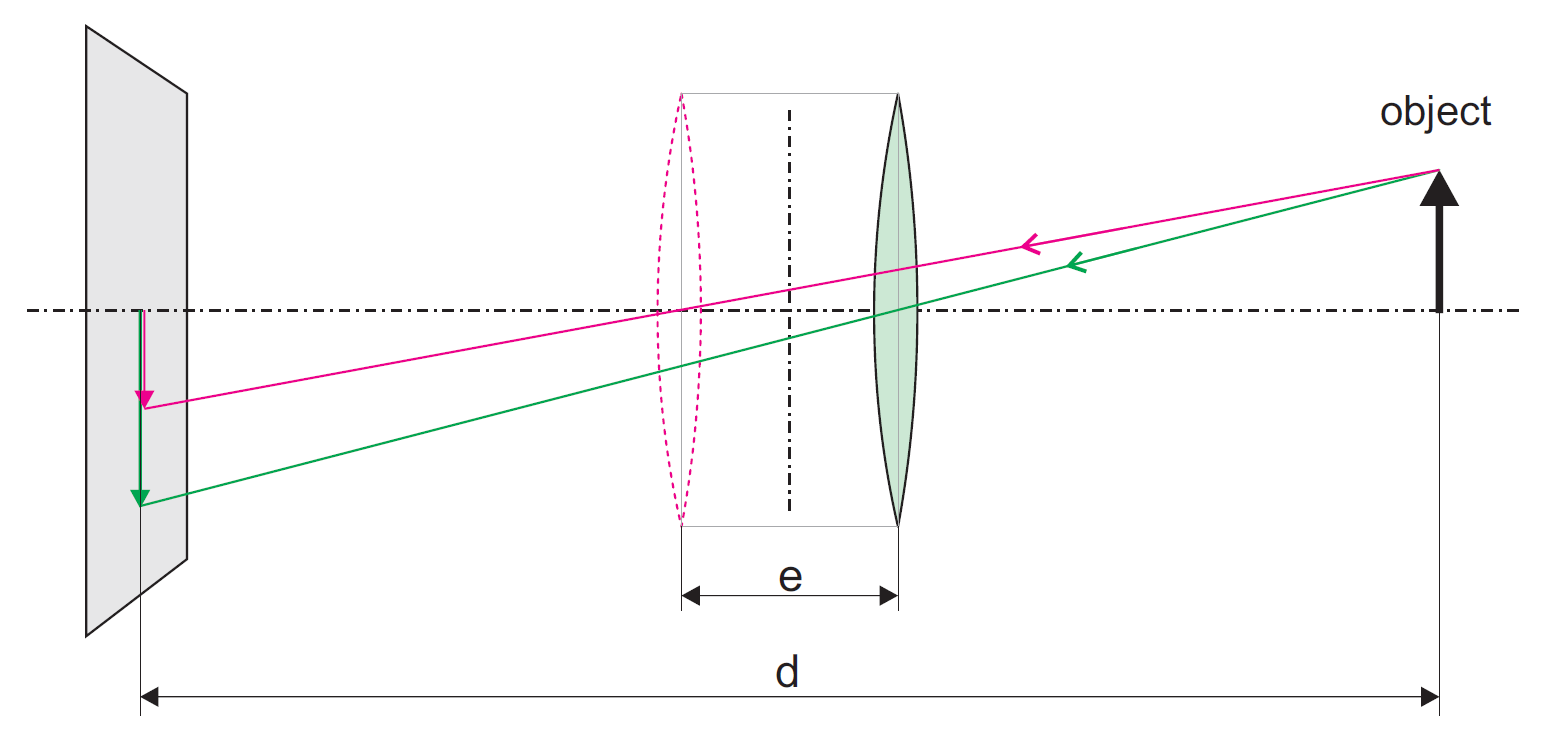
\includegraphics[width=0.8\textwidth]{img/bessel.PNG}
	\caption{Descriptive image\cite{manual} of the Bessel method to determine the focal length.}
	\label{fig::bessel}
\end{figure}


\subparagraph{Measuring diverging lenses}
\label{chap::div}
To measure the focal length of a diverging lens $f_{div}$, we have to set a converging one with known focal length $f_{conv}$ behind it (or in front). 
Then we measure the focal length $f$ of the resulting lens system like before using the lens equation (\ref{eq::lens}).
We can now use the following equation to determine $f_{div}$:
\begin{equation}
	\frac{1}{f} = \frac{1}{f_{div}} + \frac{1}{f_{conv}} \implies f_{div} = \frac{f_{conv} f}{f_{conv} - f}
	\label{eq::div}
\end{equation}


\paragraph{Measuring wired nets}
\label{chap::net}
Here we want to measure the grating constant $g$ of a wired net.
To do that, we image the wired net to the screen using a lens with a known focal length.
As in the beginning, we try to get the sharpest image possible by adjusting the position of the lens and get $a$ and $b$ like before.
From that, we get the magnification scale $v = b/a$.
We can then measure the grid width $g'$ of the image, and calculate $g$ by using this equation:
\begin{equation}
	g = \frac{g'}{v}
	\label{eq::grid}
\end{equation}

\paragraph{Verifying Abbe's theory}
\label{chap::slit}
Abbe's image theory gives us a formula for the critical slit width $\tilde{d}$.
We want to check the accuracy of said theory by measuring $d$ ourself.
To do this, we use the same setup as before, but now we put a vertical slit with variable width in the focal plane of the lens. 
We then close the slit until the vertical bars in the image just disappear.
In order to measure the width $d$ of the slit, we do exactly the same thing as when we were measuring the wired nets. 
